\section{Literatura, zdroje a přílohy}

BAYER, T. (2008): Algoritmy v digitální kartografii. Nakladatelstvtví Karolinum, Praha.

BAYER, T. (2026): Konvexní obálka množiny bodů. Přednáška.
Katedra aplikované geoinformatiky a kartografie. Přírodovědecká fakulta UK (cit. 3. 4. 2026). Dostupné z: \url{https://web.natur.cuni.cz/~bayertom/images/courses/Adk/adk4_new.pdf}.

\vspace{2\baselineskip}

\subsubsection*{Přílohy s ukázkami výsledků jednotlivých metod}
\begin{figure}[h!]
    \centering
    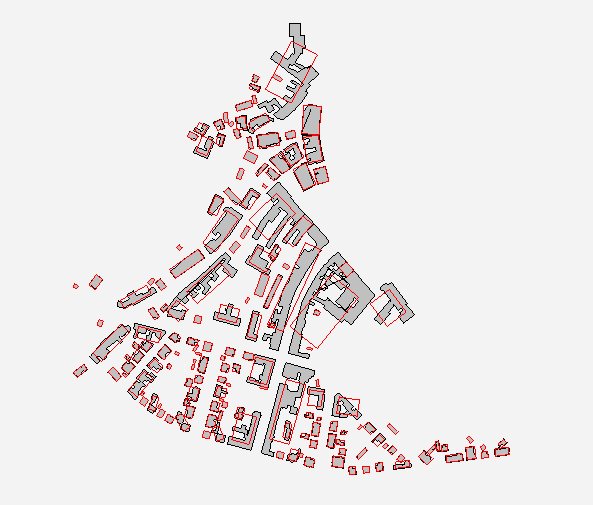
\includegraphics[width=0.9\linewidth]{figures/MBR_SM.png}
    \caption{Printscreen výsledků generalizace metodou MBR nad daty ze starého města.}
    \label{fig:obr1}
\end{figure}
\begin{figure}[h!]
    \centering
    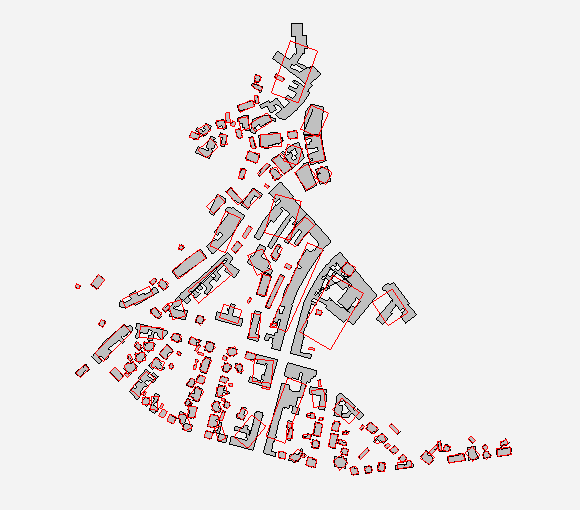
\includegraphics[width=0.9\linewidth]{figures/PCA_SM.png}
    \caption{Printscreen výsledků generalizace metodou PCA nad daty ze starého města.}
    \label{fig:obr1}
\end{figure}
\begin{figure}[h!]
    \centering
    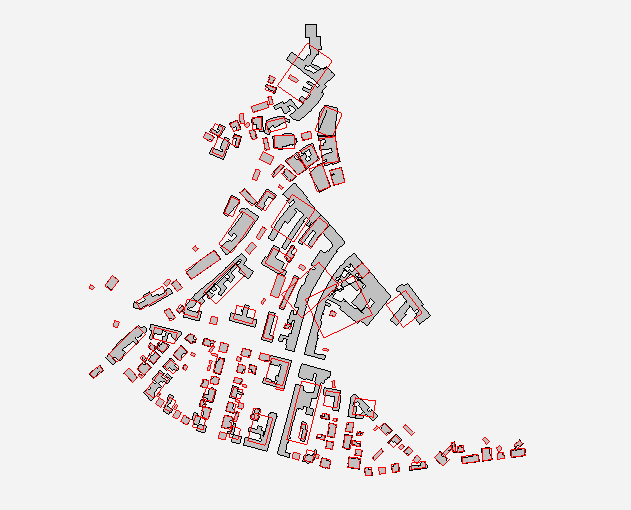
\includegraphics[width=0.9\linewidth]{figures/LongestEdge_SM.png}
    \caption{Printscreen výsledků generalizace metodou Longest edge nad daty ze starého města.}
    \label{fig:obr1}
\end{figure}
\begin{figure}[h!]
    \centering
    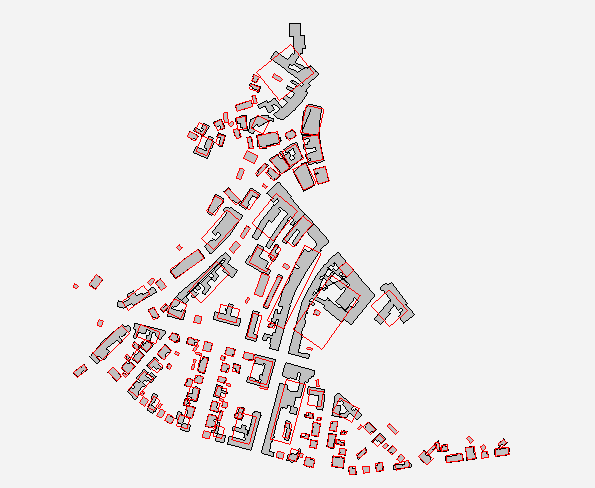
\includegraphics[width=0.9\linewidth]{figures/WallA_SM.png}
    \caption{Printscreen výsledků generalizace metodou Wall Average nad daty ze starého města.}
    \label{fig:obr1}
\end{figure}
\begin{figure}[h!]
    \centering
    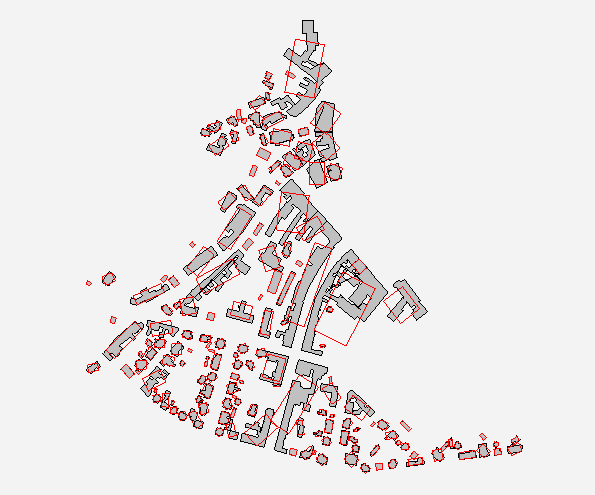
\includegraphics[width=0.9\linewidth]{figures/WBisector_SM.png}
    \caption{Printscreen výsledků generalizace metodou Weighted Bisector nad daty ze starého města.}
    \label{fig:obr1}
\end{figure}
\begin{figure}[h!]
    \centering
    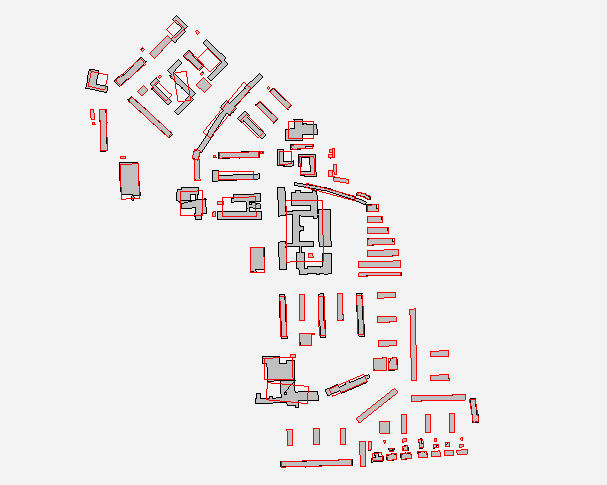
\includegraphics[width=0.9\linewidth]{figures/MBR_Sidliste.png}
    \caption{Printscreen výsledků generalizace metodou MBR nad daty ze sídliště.}
    \label{fig:obr1}
\end{figure}
\begin{figure}[h!]
    \centering
    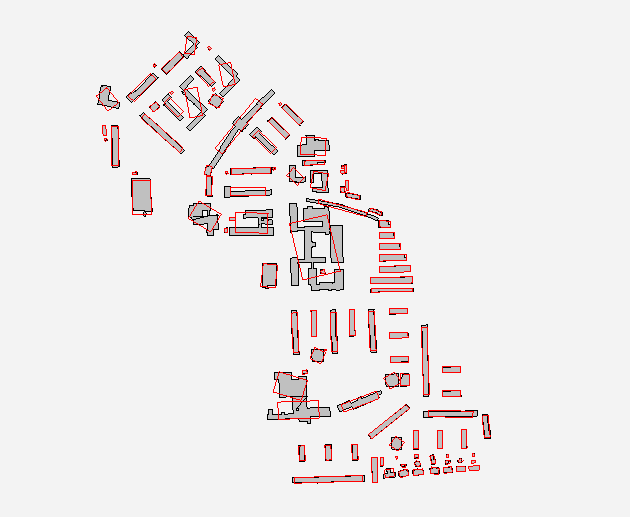
\includegraphics[width=0.9\linewidth]{figures/PCA_Sidliste.png}
    \caption{Printscreen výsledků generalizace metodou PCA nad daty ze sídliště.}
    \label{fig:obr1}
\end{figure}
\begin{figure}[h!]
    \centering
    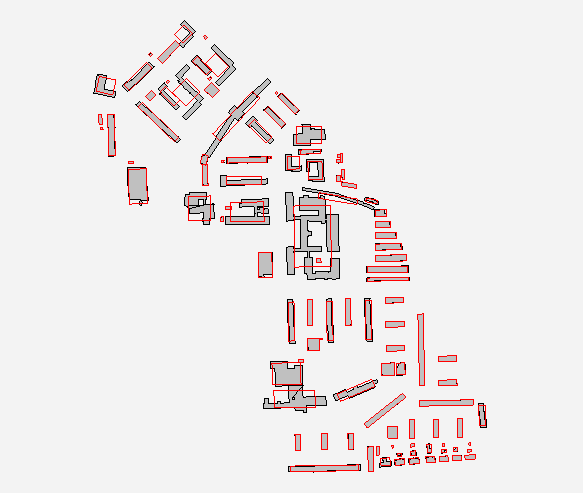
\includegraphics[width=0.9\linewidth]{figures/LongestEdge_Sidliste.png}
    \caption{Printscreen výsledků generalizace metodou Longest edge nad daty ze sídliště.}
    \label{fig:obr1}
\end{figure}
\begin{figure}[h!]
    \centering
    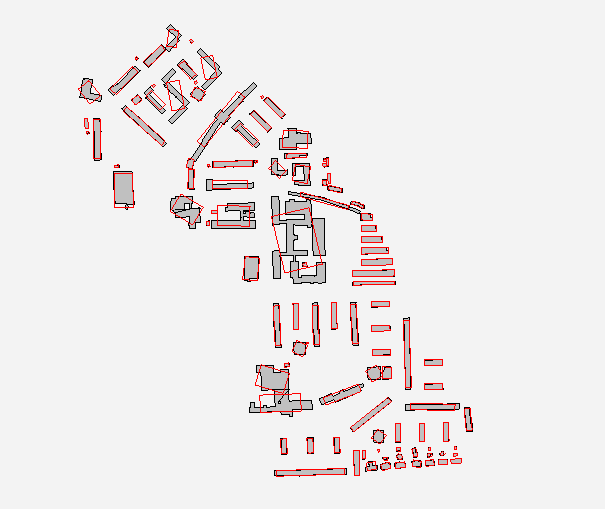
\includegraphics[width=0.9\linewidth]{figures/WallA_Sidliste.png}
    \caption{Printscreen výsledků generalizace metodou Wall Average nad daty ze sídliště.}
    \label{fig:obr1}
\end{figure}
\begin{figure}[h!]
    \centering
    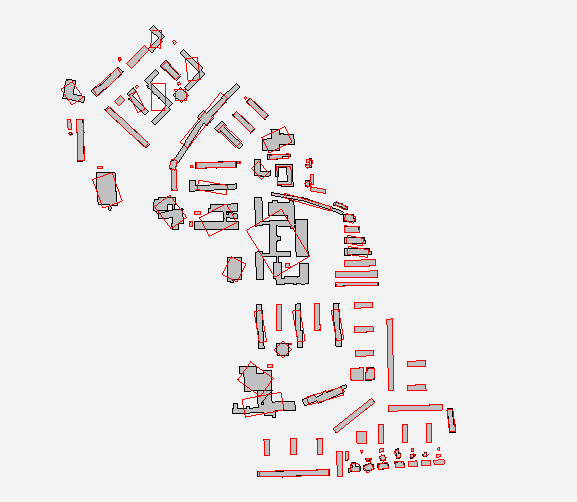
\includegraphics[width=0.9\linewidth]{figures/WBisector_Sidliste.png}
    \caption{Printscreen výsledků generalizace metodou Weighted Bisector nad daty ze sídliště.}
    \label{fig:obr1}
\end{figure}
\begin{figure}[h!]
    \centering
    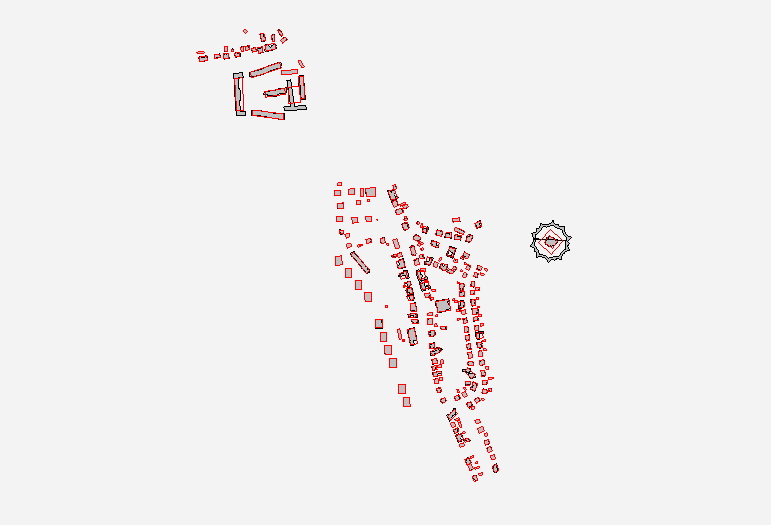
\includegraphics[width=0.9\linewidth]{figures/MBR_IZ.png}
    \caption{Printscreen výsledků generalizace metodou MBR nad daty z izolované zástavby.}
    \label{fig:obr1}
\end{figure}
\begin{figure}[h!]
    \centering
    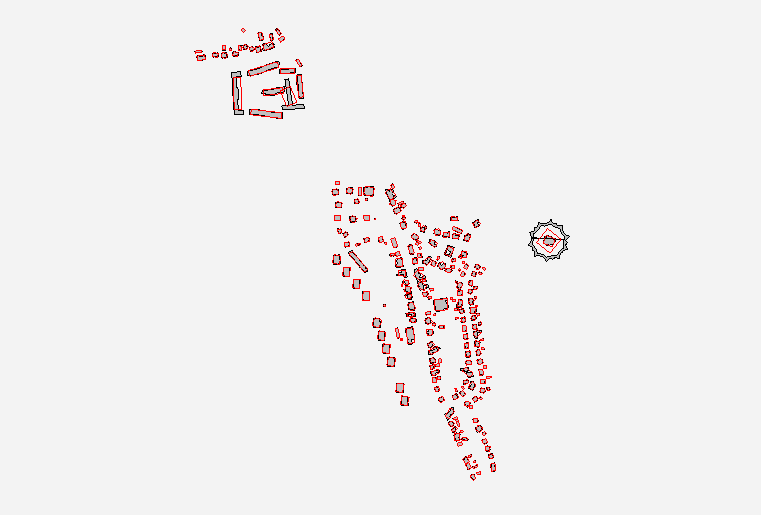
\includegraphics[width=0.9\linewidth]{figures/PCR_IZ.png}
    \caption{Printscreen výsledků generalizace metodou PCA nad daty z izolované zástavby.}
    \label{fig:obr1}
\end{figure}
\begin{figure}[h!]
    \centering
    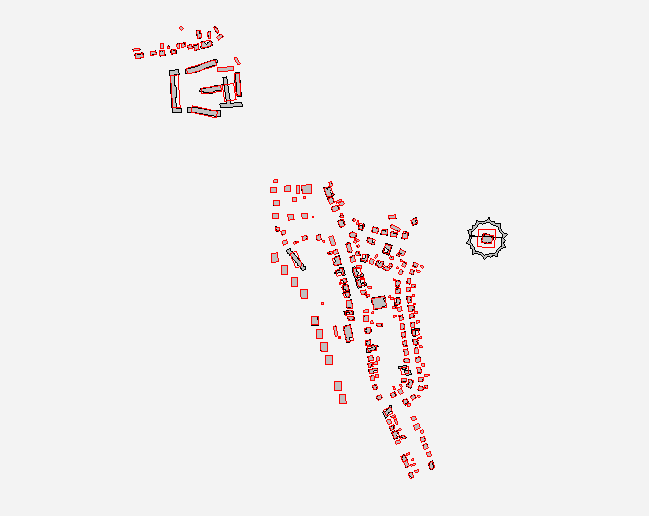
\includegraphics[width=0.9\linewidth]{figures/LongestEdge_IZ.png}
    \caption{Printscreen výsledků generalizace metodou Longest edge nad daty z izolované zástavby.}
    \label{fig:obr1}
\end{figure}
\begin{figure}[h!]
    \centering
    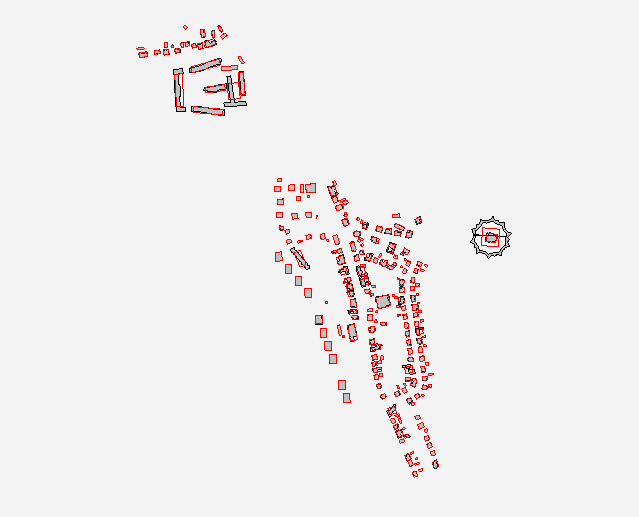
\includegraphics[width=0.9\linewidth]{figures/WallA_IZ.png}
    \caption{Printscreen výsledků generalizace metodou Wall Average nad daty z izolované zástavby.}
    \label{fig:obr1}
\end{figure}
\begin{figure}[h!]
    \centering
    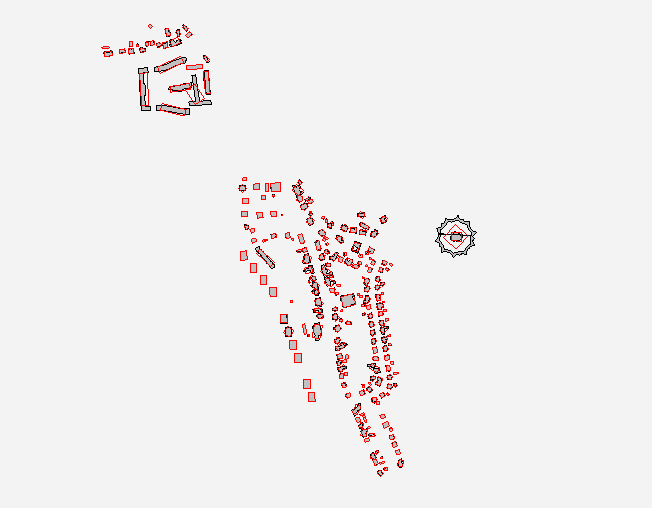
\includegraphics[width=0.9\linewidth]{figures/WBisector_IZ.png}
    \caption{Printscreen výsledků generalizace metodou Weighted Bisector nad daty z izolované zástavby.}
    \label{fig:obr1}
\end{figure}


